\documentclass[11pt,a4paper]{article}
\usepackage{tikz}
\usetikzlibrary{arrows.meta,positioning}
\usepackage{tabularx}
\usepackage{amsmath,amssymb,amsthm}
\usepackage{geometry}
\geometry{margin=1in}
\usepackage{hyperref}
\usepackage{graphicx}
\usepackage{setspace}
\onehalfspacing

\title{\textbf{Paper A-11: Earth Collapse:\\ A Constraint-Driven Flux Dynamics (CDFD) Perspective}}
\author{Steve Bico Mujjabi, MD\\
\small Independent Researcher\\
\small Founder, Vura Labs\\
\small Kampala, Uganda\\
\small ORCID: 0009-0001-0556-5516}
\date{August 2026}

\begin{document}
\maketitle

% BEGIN SHARED-METHODS POINTER
\noindent\textit{Shared Part IV notation and evidence boundaries are defined in \path{PART_IV_METHODS_AND_CLAIM_BOUNDARY.md}. This paper states only its local observables, comparison, and failure conditions.}
% END SHARED-METHODS POINTER


\begin{abstract}
This paper develops a falsifiable CDFD/AFL model of Earth Collapse. It maps compound climatic, ecological, geophysical, and human forcing to driving flux $\Phi$, shrinking buffers, connectivity bottlenecks, and finite recovery capacity to active constraint $C$, refugia, redundancy, migration, repair, and coordinated response to responsiveness $S$, and cumulative damage, lost diversity, degraded infrastructure, and prior shocks to structural memory $M_s$. The target outcome is cascade size, tipping risk, loss, and recovery, tested against paleorecords, hazard databases, ecological monitoring, infrastructure records, and recovery series. The paper treats universality as a shared model architecture rather than an assertion that unlike systems have the same material mechanism. It states the negative result that would make the mapping unnecessary and places the domain claim inside the cumulative CDFD programme and its reproducible runtime boundary.
\end{abstract}

\section{Introduction}

Earth maintains a delicate thermodynamic equilibrium, venting just enough solar radiation back into space to support liquid water. This equilibrium is actively regulated by the biosphere and lithosphere, which act as a massive, distributed thermostat drawing carbon out of the atmosphere.

If this thermostat fails, a planet enters a runaway greenhouse state, as evidenced by Venus. In CDFD terms, a runaway greenhouse effect is not merely an increase in temperature; it is the total, unrecoverable topological locking of a planetary membrane.

\section{The Planetary Adaptive Surface}
We apply the Adaptive Operating Ratio to the entire planetary atmosphere:
\begin{equation}
    \Psi_s = \left( \frac{\Phi}{C} \right) \cdot S \cdot M_s
\end{equation}

For a planetary climate system:
\begin{itemize}
    \item \textbf{Flux ($\Phi$)}: The incoming solar radiation (insolation) and the outward flow of longwave infrared radiation.
    \item \textbf{Constraint ($C$)}: Greenhouse gas concentrations (like $CO_2$ and $CH_4$) that act as an optical constraint, physically blocking the outward flux of heat.
    \item \textbf{Responsiveness ($S$)}: The capacity of carbon sinks (oceans, forests, and silicate weathering) to dynamically absorb excess carbon and reduce the constraint $C$.
    \item \textbf{Memory ($M_s$)}: The geologic and atmospheric equilibrium state. If oceans boil, the planet permanently "remembers" the loss of its primary heat sink, locking the system into a high-constraint topology.
\end{itemize}

\subsection{The Venusian Attractor and Runaway Collapse}
On a stable Earth, an increase in solar flux $\Phi$ or a spike in greenhouse constraints $C$ is met by an increase in weathering and biological uptake ($S$). The system flexes, maintaining $\Psi_s \approx 1$.

However, if $C$ rises too rapidly (e.g., massive industrial emissions or continental flood basalts), the surface temperature spikes. This heat destroys the planet's responsiveness $S$. Forests burn (releasing more $C$), and the oceans warm, reducing their ability to absorb $CO_2$ and eventually evaporating.

As water vapor (a potent greenhouse gas) floods the atmosphere, the constraint $C$ reaches a critical, runaway threshold. The physical mechanisms that could lower $C$ are entirely destroyed. The systemic memory ($M_s$) permanently locks the atmosphere into a hyper-constrained state. The outward thermal flux $\Phi$ is entirely blocked. The adaptive ratio crashes ($\Psi_s \ll 1$), and the planet transitions to the Venusian attractor---a dead, topologically locked pressure cooker from which no biological life can emerge.



\section{Measurement Layer}

% BEGIN PART IV MAJOR CROSS-DOMAIN UPGRADE
\section{Cross-Domain Model Upgrade: Mechanism, Scale, and Tests}

\subsection{Observable Translation}

The paper-specific translation begins with an observable chain rather than a
verbal analogy. For Earth Collapse, the proposed drive is compound climatic, ecological, geophysical, and human forcing.
The active limitation is shrinking buffers, connectivity bottlenecks, and finite recovery capacity. Responsiveness is carried by
refugia, redundancy, migration, repair, and coordinated response, while retained state is represented by
cumulative damage, lost diversity, degraded infrastructure, and prior shocks. The outcome to explain is cascade size, tipping risk, loss, and recovery.

\begin{table}[htbp]
\centering
\small
\caption{Operational CDFD/AFL map for Paper A-11.}
\begin{tabularx}{\textwidth}{|l|X|X|}
\hline
\textbf{Term} & \textbf{Paper-specific observable meaning} & \textbf{Measurement question} \\
\hline
$\Phi$ & compound climatic, ecological, geophysical, and human forcing & What rate, load, gradient, or demand enters the focal system? \\
\hline
$C$ & shrinking buffers, connectivity bottlenecks, and finite recovery capacity & Which measured bottleneck limits transfer, function, or recovery? \\
\hline
$S$ & refugia, redundancy, migration, repair, and coordinated response & Which process changes effective capacity or reroutes the load? \\
\hline
$M_s$ & cumulative damage, lost diversity, degraded infrastructure, and prior shocks & Which retained state makes equal present loads produce different futures? \\
\hline
$Y$ & cascade size, tipping risk, loss, and recovery & Which outcome is predicted out of sample, with uncertainty? \\
\hline
\end{tabularx}
\end{table}

\begin{figure}[htbp]
\centering
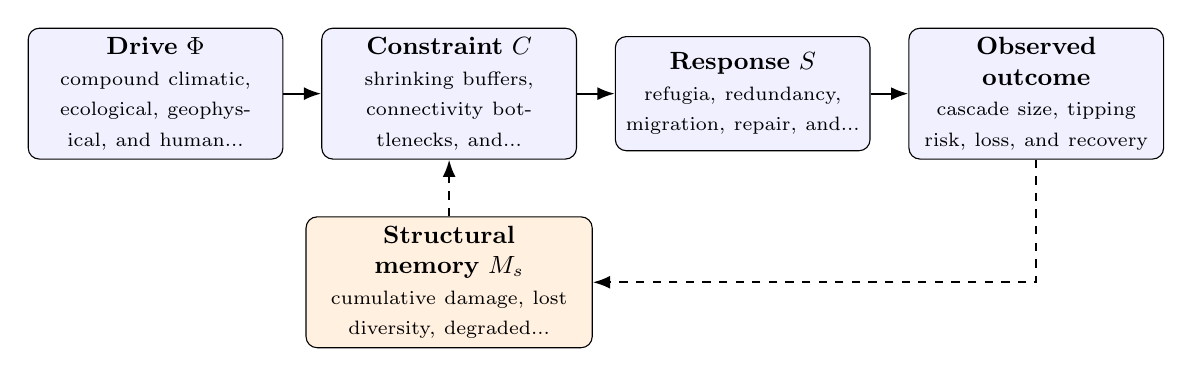
\begin{tikzpicture}[
    node distance=0.48cm,
    every node/.style={font=\small},
    box/.style={draw, rounded corners, align=center, minimum height=1.45cm, text width=3.0cm, fill=blue!6},
    memory/.style={draw, rounded corners, align=center, minimum height=1.25cm, text width=3.4cm, fill=orange!12},
    flow/.style={-{Latex[length=2.2mm]}, thick},
    feedback/.style={-{Latex[length=2.2mm]}, thick, dashed}
]
\node[box] (drive) {\textbf{Drive $\Phi$}\\\scriptsize compound climatic, ecological, geophysical, and human...};
\node[box, right=of drive] (constraint) {\textbf{Constraint $C$}\\\scriptsize shrinking buffers, connectivity bottlenecks, and...};
\node[box, right=of constraint] (response) {\textbf{Response $S$}\\\scriptsize refugia, redundancy, migration, repair, and...};
\node[box, right=of response] (outcome) {\textbf{Observed outcome}\\\scriptsize cascade size, tipping risk, loss, and recovery};
\node[memory, below=0.72cm of constraint] (memory) {\textbf{Structural memory $M_s$}\\\scriptsize cumulative damage, lost diversity, degraded...};
\draw[flow] (drive) -- (constraint);
\draw[flow] (constraint) -- (response);
\draw[flow] (response) -- (outcome);
\draw[feedback] (outcome.south) |- (memory.east);
\draw[feedback] (memory.north) -- (constraint.south);
\end{tikzpicture}
\caption{Paper A-11 observable CDFD/AFL architecture for Earth Collapse. Solid arrows give the proposed forward chain; dashed arrows make history-dependent feedback explicit.}
\label{fig:a11-architecture}
\end{figure}

\subsection{Paper-Specific Causal Hypothesis}

For this paper, the hypothesized causal sequence is specific. A change in
compound climatic, ecological, geophysical, and human forcing arrives faster than refugia, redundancy, migration, repair, and coordinated response can compensate.
This raises or redistributes shrinking buffers, connectivity bottlenecks, and finite recovery capacity. If the load persists,
the retained state encoded by cumulative damage, lost diversity, degraded infrastructure, and prior shocks changes the next response, so a later event of equal
magnitude can produce a different trajectory in cascade size, tipping risk, loss, and recovery. The
scientific task is to estimate that sequence against the best ordinary model of
the domain, not merely to redescribe the outcome after it occurs.

\subsection{Cross-Scale Translation Without Mechanistic Erasure}

For the Earth systems family, the cross-domain translation compares coupled transport, finite environmental capacity, buffering, and retained landscape or ecosystem state. It cannot erase conservation laws, geometry, or scale; it must expose where those domain equations create comparable overload and recovery structures. \cite{Holling1973,Turing1952,BakTangWiesenfeld1987}
The required scale declaration for this paper is minutes to millennia; local failures to planetary cascades. At short
scales, the key question is whether the incoming drive is transmitted,
buffered, or diverted. At intermediate scales, response changes effective
capacity and network exposure. At long scales, retained structure can alter the
state space itself. A result is genuinely cross-scale only when the aggregation
rule is stated and the same conclusion is not an artifact of averaging.

\subsection{Evidence Ladder and Discriminating Tests}

\begin{table}[htbp]
\centering
\small
\caption{Evidence ladder for Paper A-11. Each rung can fail independently.}
\begin{tabularx}{\textwidth}{|p{0.17\textwidth}|X|X|}
\hline
\textbf{Test} & \textbf{Design} & \textbf{Discriminating result} \\
\hline
Proxy audit & Measure paleorecords, hazard databases, ecological monitoring, infrastructure records, and recovery series and preregister how each record maps to $\Phi$, $C$, $S$, $M_s$, and $Y$. & The mapping fails if proxies are non-identifiable, circular, or change meaning across cases. \\
\hline
Load ramp & Apply or observe two individually tolerable shocks applied in close succession while estimating the dominant constraint and response time. & A threshold claim requires a reproducible nonlinear change and uncertainty bounds, not a visually chosen breakpoint. \\
\hline
Recovery and memory & Match present load across units with different histories, then compare recovery paths. & The memory claim requires history-dependent divergence after current conditions are controlled. \\
\hline
Model comparison & Compare the baseline domain model with and without the CDFD/AFL state variables using held-out data. & The paper's stated falsifier is: compound history does not change the response once present load is controlled. \\
\hline
\end{tabularx}
\end{table}

\subsection{Research Programme and Boundary Conditions}

The immediate research programme has four steps. First, construct a documented
dataset from paleorecords, hazard databases, ecological monitoring, infrastructure records, and recovery series and retain raw units before normalization.
Second, fit a baseline domain model and report its calibration and out-of-sample
error. Third, add the smallest identifiable CDFD/AFL state extension and test
whether it improves prediction of cascade size, tipping risk, loss, and recovery. Fourth, repeat the
analysis across the declared scale range and publish negative cases as part of
the cross-domain translation audit.

% END PART IV MAJOR CROSS-DOMAIN UPGRADE

\section{Conclusion}
Planetary collapse is the ultimate manifestation of Adaptive Flux Limitation on a macro scale. A planet is a living membrane that must maintain structural elasticity ($S$) to survive thermodynamic flux. By analyzing climate change (global $\Phi$ drive overload) through CDFD, we model that once the Earth's biological and oceanographic responsiveness is exhausted, the topological slide into Venusian necrosis is a severe candidate failure mode.
\section*{Conflict of Interest} The author declares no conflict of interest.
\section*{Data Availability}
Part-specific runtime diagnostics are under each Part's \path{outputs/} directory.

Release-wide code: \path{Part_E_Synthesis/supplementary/}.

Generated summaries: \path{Part_E_Synthesis/outputs/}.

Figures: \path{Part_E_Synthesis/figures/}.


\section{Reference Layer}
\bibliographystyle{plain}
\bibliography{universal_afl_references}
\end{document}
